\documentclass[a4paper]{article}
\usepackage[utf8]{inputenc}
\usepackage[T1]{fontenc}
\usepackage[slovene]{babel}
\usepackage{lmodern}
\usepackage{hyperref}
\usepackage{blindtext}
\usepackage{amssymb}  
\usepackage{listings} %python koda
\usepackage{graphicx}
\usepackage{tabularx}
\usepackage{tikz}
\lstset{%
   breaklines=true
}

\begin{document}

\begin{titlepage}
\center
\textsc{\LARGE Univerza v Ljubljani}\\[0.5cm]
\textsc{\Large Fakulteta za matematiko in fiziko}\\[0.5cm]

{\huge\bfseries Problem k-centrov}\\[0.4cm]


\vfill\vfill\vfill

{ Filip Nose in Anja Plesec}

{ Januar, 2021}

\vfill

\end{titlepage}

\tableofcontents

\newpage

\section{Uvod}
V poročilu bova predstavila problem k-centrov in kodo s katero sva ta problem rešila. Na začetku bova podrobneje opisala problem in kakšni so bili najini cilji, v nadaljevanju pa bova kodo podrobneje komentirala in predstavila rezultate do katerih sva prišla.

\section{Naloga}
Consider the k-center problem for graphs (using the distance for graphs). Use an ILP formulation an a good ILP solver to run experiments in simple graphs, like grids (with some deleted vertices or edges) or trees. Check the running time and the optimal value depending on the different parameters (k, number of vertices or edges being removed, the size of the grid, etc.) You can also consider 3-dimensional grids or other simple families of graphs.

\section{Opis problema}

Problem k-centrov (angl. \textit{k-center problem}) govori o izbiri najboljše lokacije za $k$ objektov na tak način, da minimiziramo največjo razdaljo med mesti, kjer je povpraševanje, ter najbljižjim krajem, kjer je objekt postavljen. Primeri teh objektov so gasilski in zdravstveni domovi, skladišča, šole itd.
\par
Problem k-centrov lahko formuliramo z neusmerjenim grafom. Podan imamo graf $G = (V, E)$, kjer $V$ predstavlja množico vozlišč danega grafa, $E$ pa množico povezav. Poleg tega povezavam dodelimo pozitivne uteži $d_{ij}$, ki predstavljajo razdaljo med vozliščem $i$ in vozliščem $j$. Cilj je najti množico $S \subseteq V$  in vozlišče $v \in V$, kjer je $|S|\leq$ k, tako da bo razdalja $\max\limits_{v \in V} d(v, S)$ najmanjša.
\par
 S preprostejšimi besedami bi lahko rekli, da je cilj najti vozlišče, ki minimizira maksimalno razdaljo med vozliščem in centrom.

\vspace{\baselineskip}
\parindent 0mm
Za iskanje k-centrov bova uporabila sledeč CLP:\\

Vhodni podatki:
\begin{itemize}
\item{$d_{ij}$ \dots razdalja med vozliščem i in centrom j}
\item{$k$ \dots število centrov, ki jih moramo locirati}
\end{itemize}

Spremenljivke:
\begin{itemize}
\item{$y_{i}=1$, če je v vozlišču $i$ center}
\item{$x_{ij}= 1$, če vozlišče $i$ spada pod center $j$}
\item{$R$ \dots maksimalna razdalja med vozliščem in najbližjim centrom}
\end{itemize}

\cleardoublepage

Iščemo torej\\
$$\max R$$

pri pogojih:
$$x_{ij} \in \{0,1\} \quad\forall i,j \in V\\$$
$$y_{i} \in \{0,1\} \quad\forall i \in V \\$$
$$\sum_{j \in V} x_{ij} \geq 1 \quad \forall i \in V \\$$
$$\sum_{j \in V} y_{i} = k \\$$
$$x_{ij} \leq y_{j} \quad \forall i,j \in V \\$$
$$\sum_{j \in n} x_{ij} d_{ij} \leq R \quad\forall i \in V $$


%\begin{equation*}
%\begin{array}{rrclcl}
%\displaystyle \max R \\
%\textrm{pri pogojih}& x_{ij} \in \{0,1\}, &\quad\forall i,j \in N\\
%&y_{i} \in \{0,1\}, &\quad\forall i \in N \\
%&\sum_{j \in N} x_{ij}, \geq 1 &\quad \forall i \in V \\
%&\sum_{j \in N} y_{i} = k \\
%&x_{ij} \leq y_{j}, &\quad \forall i,j \in V \\
%&\sum_{j \in n} x_{ij} d_{ij} \leq R, &\quad\forall i \in V
%\end{array}
%\end{equation*}



\section{Cilji}
Pri najinem projektu sva se osredotočila predvsem na mreže, katerim smo odstranili poljubna vozlišča in poljubne povezave. Napisala sva tudi kodo za drevesa in gozdove.
Najin cilj je bil, da ugotoviva, kako se spreminja čas delovanja in optimalna vrednost ob spreminjanju:
\begin{itemize}
\item{števila k,}
\item{števila vozlišč ali povezav, ki sva jih odstranila in}
\item{velikosti mreže.}
\end{itemize}

\section{Koda}
V nadaljevanju so predstavljene funkcije za mreže. Podobne funkcije sva uporabljala za trodimenzionalne mreže in drevesa.

\subsection{Mreža}
V najini kodi sva najprej definirala funkcijo \texttt{mreza}, ki sprejme parametre m,n,a in b. S to funkcijo ustvarimo mrežo velikosti m$\times$n, v kateri pa poljubno izbrišemo naključnih a vozlov in naključnih b povezav.\\
%Podobne funkcije sva uporabila tudi za drevesa in trodimenzionalne mreže

\begin{lstlisting}[language=Python]
def mreza(m,n,a,b):
    mreza = graphs.Grid2dGraph(m,n)
    if a > mreza.order():
        print("Za ukaz je na voljo premalo vozlov.")
    else:
        i = 0
        while i < a:
            mreza.delete_vertex(mreza.random_vertex())
            i = i+1
        i = 0
    if b > mreza.size():
        print("Za ukaz je na voljo premalo povezav.")
    else:
        while i < b:
            mreza.delete_edge(mreza.random_edge())
            i = i+1
    return mreza
\end{lstlisting}

\subsection{CLP}
V nadaljevanju sva definirala funkcijo \texttt{najkrajsa\_razdalja}, ki reši naš CLP problem. Vrne nam najkrajšo možno najdaljšo razdaljo v našem grafu, tako da razdalja od poljubnega vozlišča do najbližjega centra manjša ali enaka le tej. Funkciji moramo podati število centrov K in graf, ki ga ustvarimo s pomočjo funkcije  \texttt{mreza}.

\begin{lstlisting}[language=Python]
def najkrajsa_razdalja(G, st_centrov):
    K = st_centrov
    razdalje = G.distance_all_pairs()

    p = MixedIntegerLinearProgram(maximization=False)
    x = p.new_variable(binary=True)
    y = p.new_variable(binary=True)

    p.set_objective(p['R'])

    for u in G:
        p.add_constraint(sum(x[u, v] for v in G) == 1)
       
    p.add_constraint(sum(y[v] for v in G) == K)

    for u in G:
        for v in G:
            p.add_constraint(x[u, v] <= y[v])

    for u in G:
        for v in G:
            if v in razdalje[u]:
                p.add_constraint(razdalje[u][v] * x[u, v] <= p['R'])
            else:
                p.add_constraint(x[u, v] == 0)
    max_razdalja = p.solve()
    skladisca = [k for k, v in p.get_values(y).items() if v == 1]
    return round(max_razdalja)
\end{lstlisting}

Od tu naprej so definirane funkcije, ki sva jih uporabila za izvajanje poskusov.

\subsection{Optimalna vrednost v odvisnosti od k in velikosti kvadratne mreže}
Zanima nas kako se spreminja povprečna optimalna vrednost R, ko spreminjamo velikost mreže in število centrov k.
\par
Funkcija nam vrne matriko, kjer element $a_{ij}$ predstavlja povprečno optimalno vrednost R (za n ponovitev) pri mreži $i \times i$, ki ima $j$ centrov. Lahko povemo tudi koliko vozlišč in/ali povezav naj bo pri tem izbrisanih izbrisanih (za vse velikosti matrik enako št. izbrisanih vozlišč $a$ in število izbrisanih povezav $b$).

\vspace{\baselineskip}

Velikost mreže narašča od 3$\times$3 do n$\times$n.\\
K-ji naraščajo od 1 do max\_k.\\

Koda je podobna tudi za mreže, kjer spreminjamo samo eno dimenzijo: m$\times$3 do m$\times$n, ki pa ni vključena v poročilo.

\begin{lstlisting}[language=Python]
def R_v_odvisnosti_od_velikosti_kvadratne_mreze_in_k(n,a,b,max_k,stevilo_ponovitev):
    seznam = [] # i-ti element tega seznama pove povprecne R-je za razlicne k-je za ixi matriko
    for i in range(6, n+1):
        seznam1 = [] #seznam povprecnega R za stevilo_centrov = j
        for j in range(1, max_k + 1):
            seznam2 = []
            for p in range(stevilo_ponovitev):
                G = mreza(i,i,a,b)
                stevilo_komponent = connected_components_number(G)
                if stevilo_komponent <= j: #st. komponent <= k (st.centrov) (j)
                    razdalja = round(najkrajsa_razdalja(G, j))
                    seznam2.append(razdalja)
                else:
                    seznam2.append(None)

            vsota = 0
            stevec = 0
            povprecje = 0
            for v in range(len(seznam2)):
                if seznam2[v] != None:
                    vsota += seznam2[v]
                    stevec += 1
            if stevec == 0:
                povprecje = None
            else:
                povprecje = vsota/stevec

            seznam1.append(povprecje)

        seznam.append(seznam1)

    return seznam
\end{lstlisting}

\subsection{Optimalni čas v odvisnosti od k in velikosti mreže}
Za računanje časov prejšnji kodi pri izračunu R-a dodamo:
\begin{lstlisting}[language=Python]
zacetni = time.time()
razdalja = round(najkrajsa_razdalja(G, j))
koncni = time.time() - zacetni
seznam2.append(koncni)
\end{lstlisting}

Vrne matriko: element $a_{ij}$ pove povprecni čas izvajanja (za n ponovitev) pri mreži $i\times i$, ki ima $j$ centrov.\\

Definirala sva tudi funkcije za izračun časov in R-jev, kjer pri fiksni velikosti spreminjamo samo k-je ali obratno. Te so uporabne za večje mreže, kjer so časi računanja precej daljši. Te funkcije ne vrnejo matrike, ampak seznam.

%\subsection{Optimalna vrednost od k}
%Prva izmed teh je bila opt\_vrednost\_k, ki nam vrne seznam optimalnih vrednosti za različno števila centrov in #
%opt\_vrednost\_za\_vec\_ponovitev, ki nam vrne seznam optimalnih vrednosti za različne k-je za več ponovitev in njihovo %povprečje. S tema dvema funkcijama, torej lahko opazujemo kako se spreminja optimalna vrednost glede na k.


%\subsection{cas izvajanja od k}
%Definirala sva tudi funkciji cas\_izvajanja\_k, ki nam vrne seznam časov izvajanja funkcije najkrajsa\_razdalja v odvisnosti od k in cas\_izvajanja\_za\_vec\_ponovitev,  ki nam vrne seznam časov izvajanja za različne k-je za več ponovitev in njihovo povprečje.

V nadaljevanju sva definirala podobne funkcije, ki nam vrnejo sezname časov izvajanja ali njihovih optimalnih vrednosti in njihova povprečja, v odvisnosti od velikosti mreže in od števila izbrisanih vozlišč in/ali izbrisanih povezav. Tu je primer za brisanje vozlišč, za brisanje povezav je funkcija podobna.


\subsection{Optimalne razdalje R v odvisnosti od spreminjanja števila izbrisanih vozlišč}
Funkcija  \texttt{R\_v\_odvisnosti\_od\_spreminjanje\_stevila\_vozlisc} za poljubno velikost mreže m$\times$n vrne povprečne optimalne vrednosti R pri različnem številu izbrisanih vozlišč. Podobna je funkcija za izračun časov izvajanja.
\par
Število izbrisanih vozlišč gre od 0 do max\_st\_izbrisanih\_vozlisc.\\
$k$ predstavlja število centrov, $b$ pa je število izbrisanih povezav, ki je konstantno.

\vspace{\baselineskip}
V \texttt{R\_v\_odvisnosti\_od\_spreminjanje\_stevila\_vozlisc} uporabimo podfunkcijo \texttt{opt\_vrednost\_vozli}, ki izvede eno ponovitev in vrne seznam, katerega i-ti element pove R za i izbrisanih vozlišč mreže m$\times$n.
\begin{lstlisting}[language=Python]
def opt_vrednost_vozli(m,n,max_st_izbrisanih_vozlisc,b,k):
    seznam_vrednosti = []
    for i in range(0,max_st_izbrisanih_vozlisc + 1):
        G = mreza(m,n,i,b)
        stevilo_komponent = connected_components_number(G)
        if stevilo_komponent <= k:
            razdalja = round(najkrajsa_razdalja(G, k))
            seznam_vrednosti.append((razdalja))
        else:
            seznam_vrednosti.append(None)
            
    return seznam_vrednosti
\end{lstlisting}

fukncija vrne opt. razdalje R glede na število odstranjenih vozlišč
FIKSNO:velikost mreze, K, st. izbrisanih povezav
SPREMINJAM: st\_izbrisanih vozlišč

\begin{lstlisting}[language=Python]
def R_v_odvisnosti_od_spreminjanje_stevila_vozlisc(m,n,max_st_izbrisanih_vozlisc,b,k,stevilo_ponovitev):
    seznam = []
    for i in range(stevilo_ponovitev):
        razdalje = opt_vrednost_vozli(m,n,max_st_izbrisanih_vozlisc,b,k)
        seznam.append(razdalje)

    povprecja = []
    for j in range(max_st_izbrisanih_vozlisc + 1):
        vsota = 0
        stevec = 0
        for i in range(stevilo_ponovitev):
            if seznam[i][j] != None:
                vsota += seznam[i][j]
                stevec += 1
        if stevec == 0:
            povprecja.append(None)
        else:
            povprecja.append(vsota/stevec)
    return seznam, povprecja
\end{lstlisting}

Koda za brisanje povezav je precej podobna tej, zato v poročilo ni vključena.

\section{Poskusi}
\subsection{Čas izvajanja}
Za na konec sva izvedla poskuse na že omenjenih funkcijah, torej kako se čas izvajanja in optimalna vrednost R spreminjata glede na večanje števila centrov(k), večanje mreže in glede na število izbrisanih vozlišč in/ali robov.\\

\subsection{Čas izvajanja pri kvadratnih matrikah}
Graf prikazuje kako se čas izvajanja spreminja glede na število centrov. Vidimo lahko, da večje kot je število centrov, daljši je čas izvajanja. Na začetku strmo narašča, za velike k-je pa se ratuje bolj in bolj konstantna. Očitna je tudi precejšnja razlika časov izvajanja pri večanju velikosti mreže. Pri mreži 3$\times$3 so časi nekaj stotink sekunde, 5$\times$5 že nekaj sekund, pri 6$\times$6 pa lahko čas merimo že v minutah.

\begin{figure}[h]
  \centering
  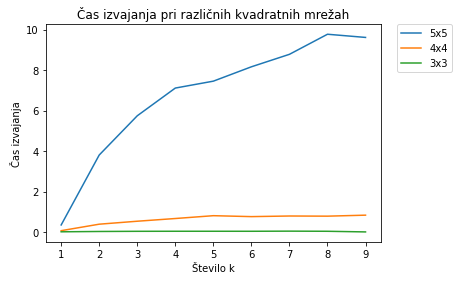
\includegraphics[width= 8cm]{cas_kvadratne_mreze}
\end{figure}
\break

\subsection{Čas in R v odvisnosti od velikost matrike in k}
\begin{figure}[h]
  \centering
  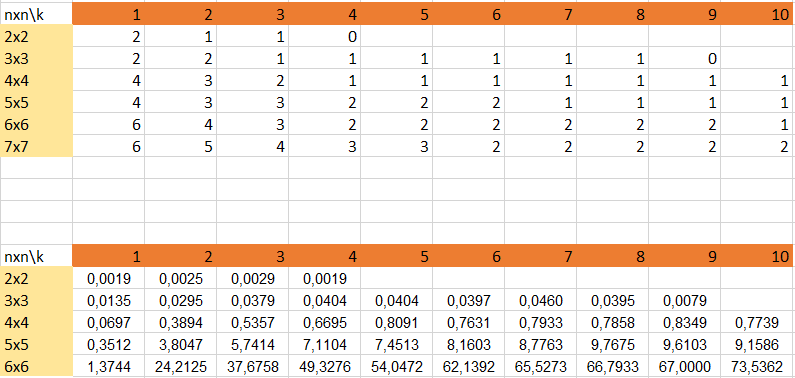
\includegraphics[width= 0.9\textwidth]{tabela_kvadratne}
\end{figure}

Spodnja grafa prikazujeta rezultate iz zgornje tabele, torej kako se čas izvajanja oz. optimalna vrednost spreminja, ko povečujemo velikost mreže in število centrov. Iz prvega grafa vidimo, da čas za velike mreže zelo hitro narašča, iz drugega pa da velikost nima tolkšnega vpliva na optimalno vrednost, kot pa število centrov.
\begin{figure}[h]
  \centering
  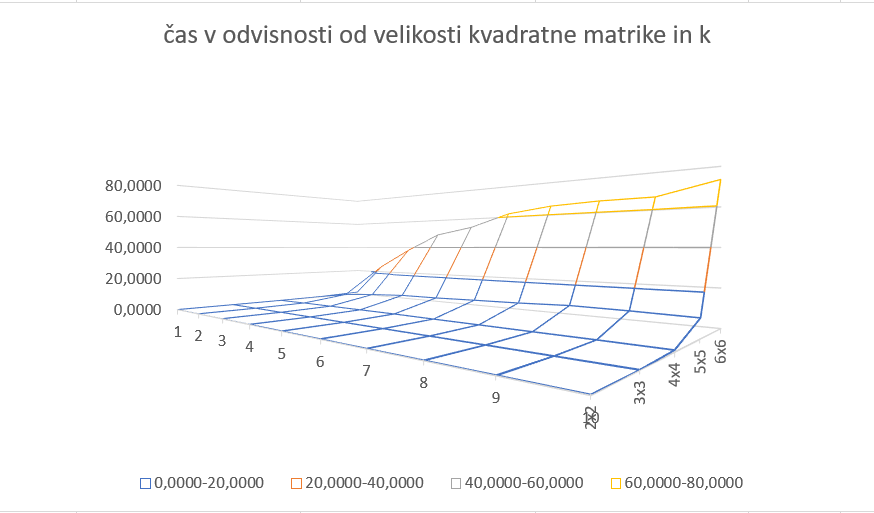
\includegraphics[width= 0.8\textwidth]{cas_3D}
\end{figure}

\newpage

\begin{figure}[h]
  \centering
  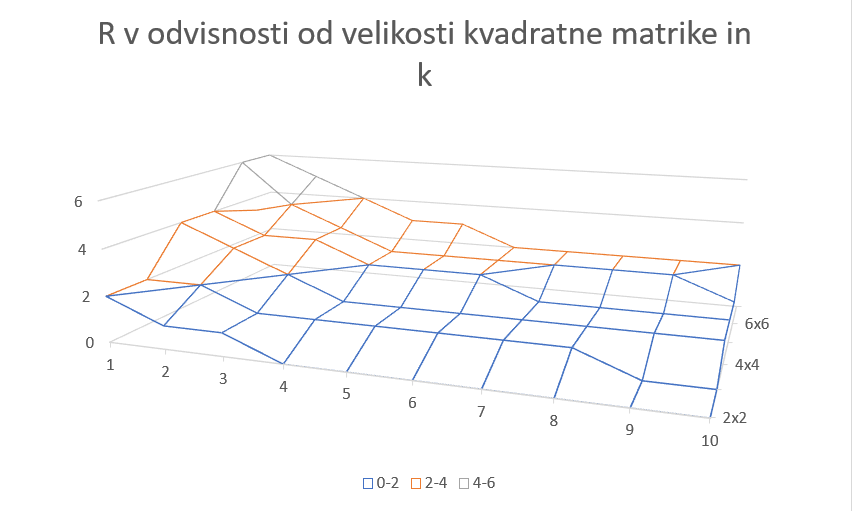
\includegraphics[width= 0.8\textwidth]{R_3D}
\end{figure}

\subsection{Čas izvajanja pri odstranjevanju vozlišč in povezav}
Iz spodnjega grafa lahko vidimo, kako čas izvajanja pada, ko odstranjujemo vozlišča. Kar je seveda smiselno, saj manj vozlišč kot ima graf, hitreje se izvede CLP koda. Prav tako če pri brisanju vozlišč graf razpade na več delov, to še toliko bolj pripomore k manjšim časom izvajanja, saj CLP občutno hitreje izračuna več manjših mrež kot eno veliko. Poskus sva izvedla na 5$\times$5 mreži, za tri različne k-je in sicer, 2,5 in 10. 
\begin{figure}[h!]
  \centering
  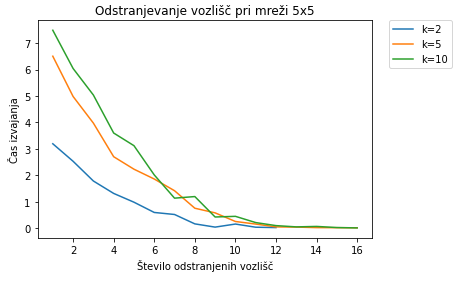
\includegraphics[width= 0.8\textwidth]{cas_vozlisca}
\end{figure}
\newpage

Graf prikazuje, kako se čas izvajanja spreminja glede na število odstranjenih povezav pri 5$\times$5 mreži za k= \{1,5,10\}. Opaziti je padanje časov, vendar precej počasneje kot pri brisanju vozlišč. To zato, ker poleg tega da je vozlišč vedno manj, vsakič ko odstranimo vozlišče odstranimo tudi vse njegove povezave, kar lahko pomeni do 4 povezav. Pri brisanju povezav so spremembe manjše, hkrati pa smo jih tu izbrisali do 10, vseh povezav pa je 40. Do skokov na grafu pride tudi zato, ker so bilo za vsako izbrisano povezavo izvedeni le 3 poskusi in bi padanje verjetno bilo bolj enakomerno, če bi teh poskusov bilo več.
\begin{figure}[h]
  \centering
  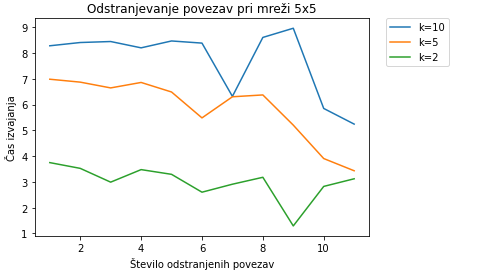
\includegraphics[width= 0.8\textwidth]{cas_povezave}
\end{figure}


\subsection{Čas in R pri pravokotnih in kvadratnih mrežah}
Na grafu je razvidno, da za primerljivo število vozlišč CLP najhitreje izračuna kvadratne mreže, bolj kot pa je mreža podolgovata, več dela ima.
\begin{figure}[h!]
  \centering
  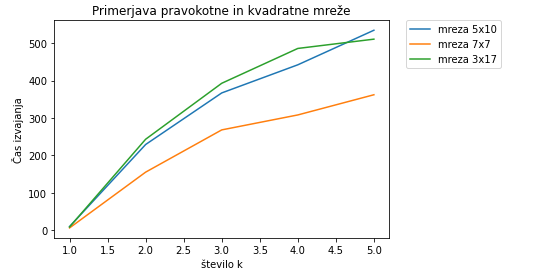
\includegraphics[width= 0.8\textwidth]{cas_pravokotna_vs_kvadratna}
\end{figure}
\newpage

Za velike k-je vidimo da so optimalne razdalje enake, razlike pa se pojavijo pri manjših k. V splošnem ne moremo reči, da za vsak k velja, da bo za bolj podolgovate mreže optimalna razdalja večja. To pokaže tudi graf pri k=2, kjer optimalna razdalja pri kvadratni mreži ni najmanjša.Zgodi se lahko torej, da si nekateri k-ji pri podolgovatih mrežah lepše razdelijo prostor, kot pri kvadratnih mrežah.

\begin{figure}[h!]
  \centering
  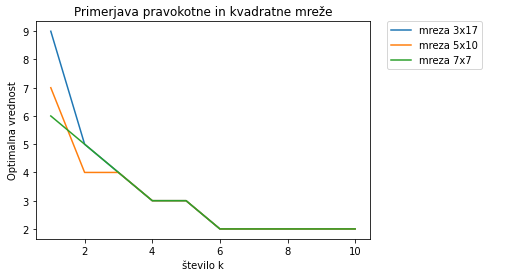
\includegraphics[width= 0.8\textwidth]{R_pravokotna_vs_kvadratna}
\end{figure}

\subsection{Optimalna vrednost pri drevesu in kvadratni mreži}
Opazimo, da je optimalna vrednost pri drevesih, ki imajo isto število vozlišč kot mreža, večja ali enaka, ne glede na število centrov.
\begin{figure}[h!]
  \centering
  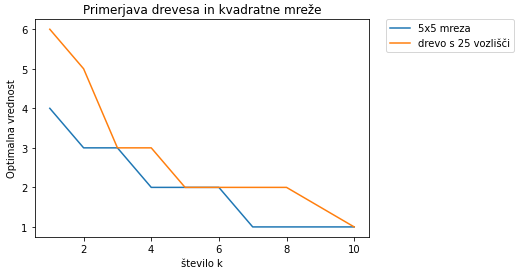
\includegraphics[width= 0.8\textwidth]{drevo_vs_kvadratna}
\end{figure}

\newpage

\subsection{Primerjava tridimenzionalne in dvodimenzionalne mreže}
Obe mreži imata 36 vozlišč. Na grafih vidimo, da so časi izvajanja pri obeh zelo podobni, razlikujeta pa se v optimalnih vrednostih. Trodimenzionalni grafi imajo pri istem k manjšo optimalno vrednost, kar je posledica boljše povezanosti vozlišč. Tu ima vozlišče lahko kar šest sosedov, v primerjavi z maksimalno štirimi sosedi pri dvodimenzionalnih mrežah.
\begin{figure}[h!]
  \centering
  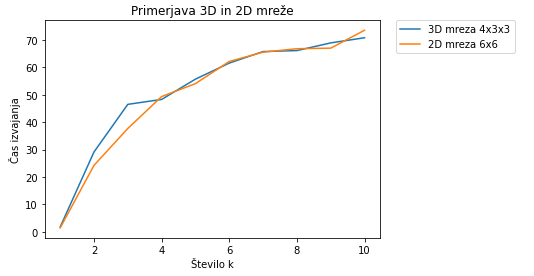
\includegraphics[width= 0.8\textwidth]{cas_3D_vs_2D}
  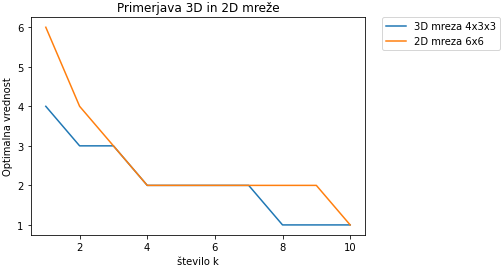
\includegraphics[width= 0.8\textwidth]{R_3D_vs_2D}
\end{figure}

\newpage


\section{Viri}

\begin{itemize}
\item Rana, R., Garg, D. (2011). An Evaluation of K-Center Problem Solving Techniques,towards Optimality. Dostopno na: https://www.longdom.org/open-access/an-evaluation-of-kcenter-problem-solving-techniques-towards-optimality-0976-4860-2-206-214.pdf?fbclid=IwAR2KDCBmif7PnRmwStiAYKnHX4Gw6UFae0h4sAo-UPN7rUaT7uRH1Ys8unc

\end{itemize}

\end{document}